%++++++++++++++++++++++++++++++++++++++++
% Don't modify this section unless you know what you're doing!
\documentclass[letterpaper,11pt]{report}
\usepackage{natbib}
\bibliographystyle{unsrtnat}
\usepackage{tabularx} % extra features for tabular environment
\usepackage{amsmath}  % improve math presentation
\usepackage{graphicx} % takes care of graphic including machinery
\usepackage[margin=1in,letterpaper]{geometry} % decreases margins
%\usepackage{cite} % takes care of citations
\usepackage[final]{hyperref} % adds hyper links inside the generated pdf file
\hypersetup{
	colorlinks=true,       % false: boxed links; true: colored links
	linkcolor=blue,        % color of internal links
	citecolor=blue,        % color of links to bibliography
	filecolor=magenta,     % color of file links
	urlcolor=blue         
}
%++++++++++++++++++++++++++++++++++++++++
\usepackage{titlesec}
\usepackage{float}
\usepackage{xcolor}
\usepackage{tcolorbox}
\usepackage{listings}

\titleformat
{\chapter} % command
[hang] % shape
{\color{blue}\bfseries\LARGE} % format
{Exp.\thechapter} % label
{0 ex} % sep
{
    \vspace{0.5 ex}
} % before-code
 

\begin{document}

\title{Astro E-Record}
\author{Darvin Raj P}
\date{}
\maketitle
\tableofcontents

\chapter{Classification of Stellar Spectra using Project CLEA}

\section{Aim}

To obtain the spectra of different stars, to determine its spectral classification and to identify the prominent
lines in it using project CLEA software.

\section{Theory}

A star’s spectrum contains information about its temperature, chemical composition, and intrinsic luminosity.Spectrograms secured with a slit spectrograph consist of a sequence of images of the slit in the light of
the star at successive wavelengths. Stellar classification is the classification of stars based on their spectral
characteristics.
\begin{figure}[H]
    \centering
    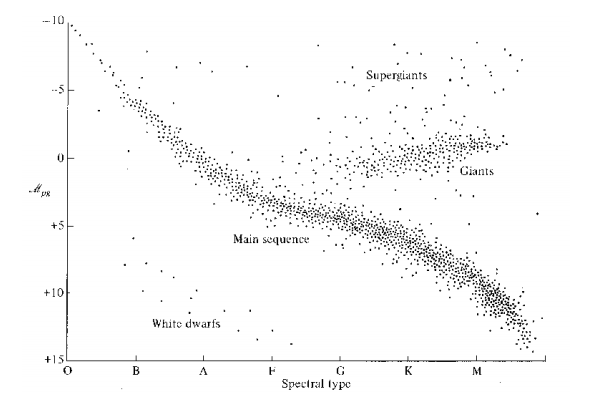
\includegraphics[scale=0.4]{spectralType.png}
    \caption{Common Spectral Types}
    \label{fig:my_label}
\end{figure}
The Morgan–Keenan (MK) system uses the letters O, B, A, F, G, K, and M, a sequence from the hottest (O type) to the coolest (M type). Each letter class is then subdivided using a numeric digit with
0 being hottest and 9 being coolest. In the MK system, a luminosity class is added to the spectral class using
Roman numerals. This is based on the width of certain absorption lines in the star’s spectrum. The figure 1
shows it in detail.
\begin{figure}[H]
    \centering
    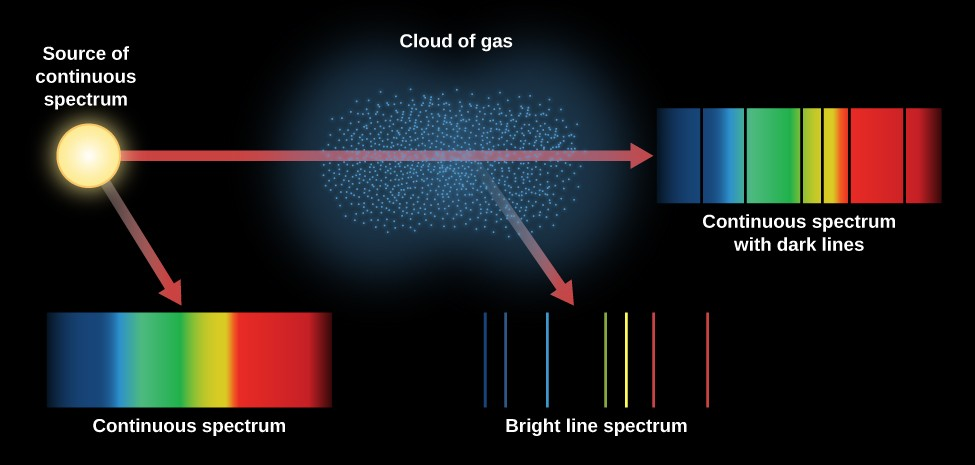
\includegraphics[scale=0.4]{OSC_Astro_05_05_TSpectra.jpg}
    \caption{Formation of star spectrum}
    \label{fig:my_label}
\end{figure}
All stellar spectra show absorption lines due to a variety of species. Spectral lines are produced by transitions of electrons within atoms or ions. The physical processes behind the formation of stellar spectra are well
enough understood to permit determinations of temperatures, densities, and chemical compositions of stellar
atmospheres. Since temperature controls ionization and excitation of the atoms, this spectral classification basically reflects a temperature sequence. This temperature sequence is also obvious from the colours of stars. An
absorption spectrum is produced when a continuum passes through ”cooler” gas. Photons of the appropriate
energies are absorbed by the atoms in the gas. Although the photons may be re-emitted, they are effectively
removed from the beam of light, resulting in a dark or absorption feature. The atmospheres of stars act as a
cooler blanket around the hotter interior of a star so that typical stellar spectra are absorption spectra. This is
clear from the figure 2

\section{Sources and Tools}

\subsection{Project CLEA}
Project CLEA a contemporary laboratory experience in astronomy develops laboratory exercises that
illustrate modern astronomical techniques using digital data and color images. Each CLEA laboratory
exercise includes a dedicated computer program. The technical guides describe file formats, user-settable
options, and algorithms used in the programs.

\subsection{VIREO}
VIREO the Virtual Educational Observatory is a simulated observatory which can access a huge database
of astronomical information, both through a set of dedicated catalogs and via on-line databases. It provides
a set of optical and infrared telescopes of various sizes along with a radio telescope. Auxiliary equipment
includes CCD and infrared imagers, an aperture photometer, a single-slit spectrometer and a multi-object
fiber-fed spectrometer, and multiple tunable radio receivers. Analysis tools are provided for astrometry,
photometry, spectrum analysis, and a variety of other purposes. VIREO provides the instructor not only
the means to carry out established CLEA exercises, but also to design new exercises and open-ended
discovery experiences that realistically simulate modern astrophysical research.


\subsection{SIMBAD}
The SIMBAD is an astronomical database that provides basic data, cross-identifications, bibliography
and measurements for astronomical objects outside the solar system. SIMBAD can be queried by object
name, coordinates and various criteria. Lists of objects and scripts can be submitted.

\section{Procedure}

\begin{itemize}
    \item Download the CLEA software particularly VIREO
    \item Login using a name and run the exercise CLassification Of Stellar Spectra.
    \item Go to Telescope and access the 0.4 meters telescope. Open the Telescope access and Switch it on.
    \item Click on Tracking and Select the Telescope option in the View menu.
    \item Go to Slew menu and select Set Coordinates. Get the coordinates of the stars whose spectra has to be
        obtained and analysed from Simbad ’http://simbad.u-strasbg.fr/simbad’ and click on OK.
    \item Click on Access button and we get the spectrum of the star in a new window. Save this spectra for further
        use.
    \item Close the Telescope access window and go to Tools and select Spectral Classification. In the new window
        that appear go to File, Unknown Spectra and click Saved spectra. Import the saved spectra.
    \item Go to File again and click Atlas of standard spectra. From the list of standard spectra that appears select
        the one that closely matches with the saved spectra. The difference can be seen by clicking File, Display
        and Show difference. This will be the spectral type of the star.
    \item In order to find the prominent lines go to File and click on Spectral line table. The table appearing gives
        the list of prominent lines out of which we can select and identify the ones needed.
\end{itemize}

\newpage

\section{Results}

The stars selected are :
\begin{itemize}
    \item Alderbaran
    \item Arcturus
    \item Bellatrix
    \item Betelgeuse
    \item Deneb
    \item HD 34500
    \item HD 51797
    \item Rigel
    \item Sirius
    \item Vega
\end{itemize}

\newline 

    \begin{figure}[H]
        \centering
        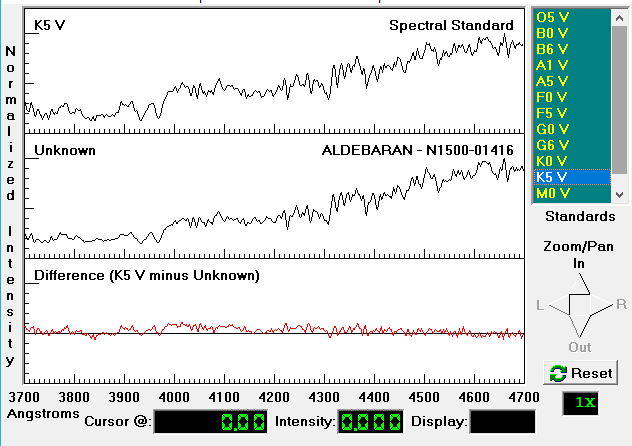
\includegraphics[scale=0.4]{Aldebaran.png}
        \caption{Aldebaran}
        \label{fig:my_label}
    \end{figure}
    \begin{figure}[H]
        \centering
        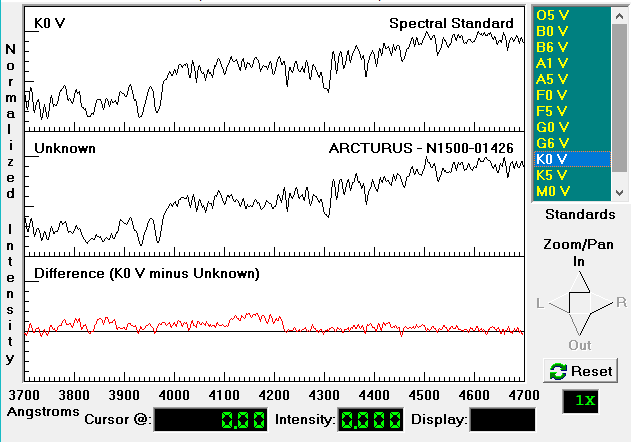
\includegraphics[scale=0.4]{Arcturus.png}
        \caption{Arcturus}
        \label{fig:my_label}
    \end{figure}
    \begin{figure}[H]
        \centering
        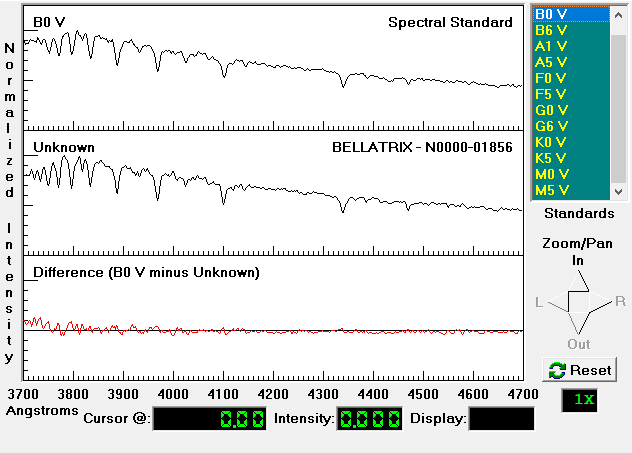
\includegraphics[scale=0.4]{Bellatrix.png}
        \caption{Bellatrix}
        \label{fig:my_label}
    \end{figure}
    \begin{figure}[H]
        \centering
        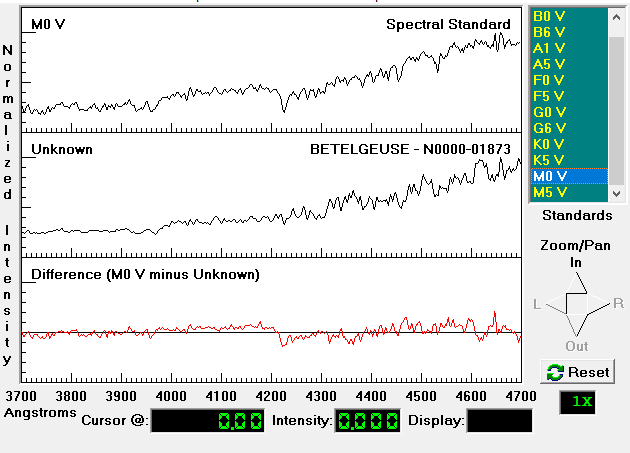
\includegraphics[scale=0.39]{Betelgeuce.png}
        \caption{Betelgeuse}
        \label{fig:my_label}
    \end{figure}
    \begin{figure}[H]
        \centering
        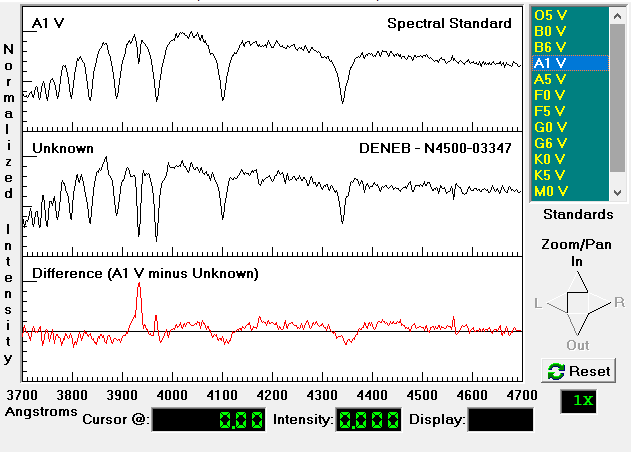
\includegraphics[scale=0.4]{Deneb.png}
        \caption{Deneb}
        \label{fig:my_label}
    \end{figure}
    \begin{figure}[H]
        \centering
        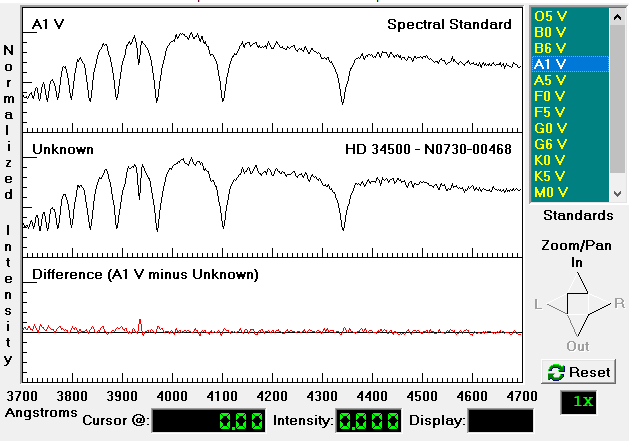
\includegraphics[scale=0.4]{HD 34500.png}
        \caption{HD 345000}
        \label{fig:my_label}
    \end{figure}
    
    \begin{figure}[H]
        \centering
        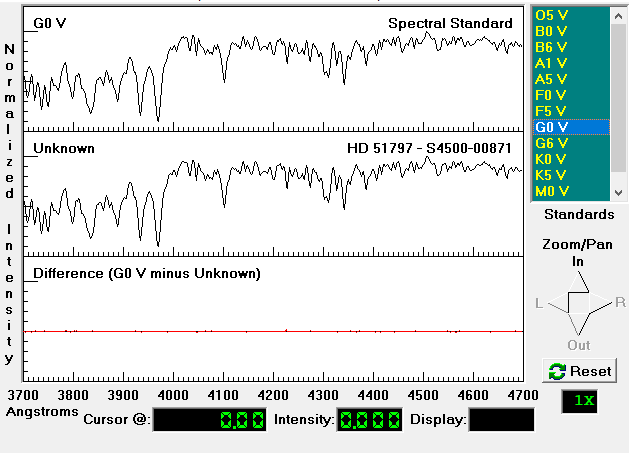
\includegraphics[scale=0.4]{HD 51797.png}
        \caption{HD 51797}
        \label{fig:my_label}
    \end{figure}
    
    \begin{figure}[H]
        \centering
        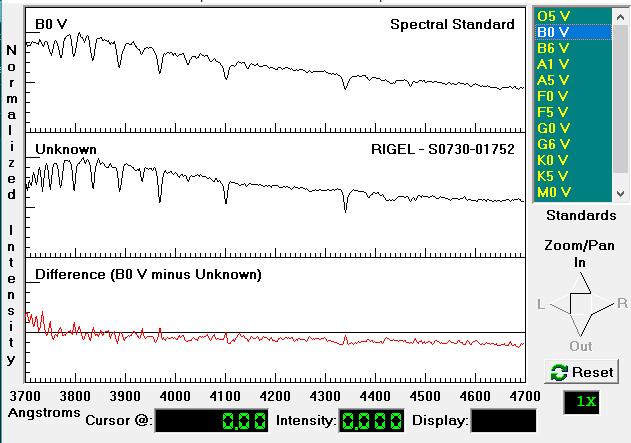
\includegraphics[scale=0.4]{Rigel.png}
        \caption{Rigel}
        \label{fig:my_label}
    \end{figure}
    
    \begin{figure}[H]
        \centering
        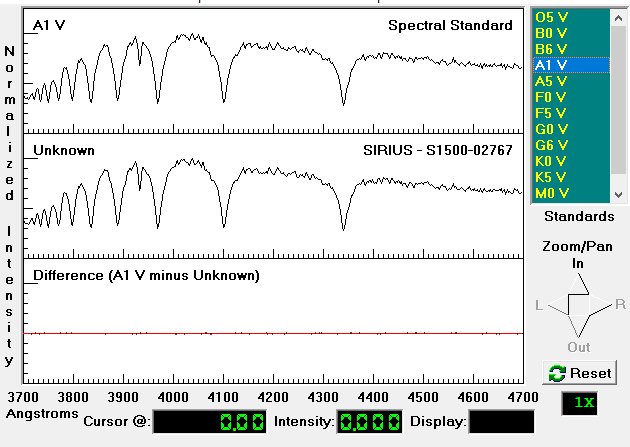
\includegraphics[scale=0.4]{Sirius.png}
        \caption{Sirius}
        \label{fig:my_label}
    \end{figure}
    
    \begin{figure}[H]
        \centering
        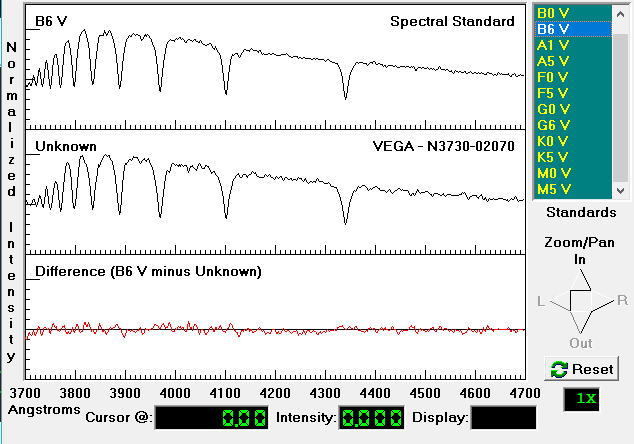
\includegraphics[scale=0.4]{Vega.png}
        \caption{Vega}
        \label{fig:my_label}
    \end{figure}
    
 \section{Observations} 
The spectral types and prominent lines of the stars above are :
    \begin{center}
        \begin{tabular}{|m{5em}|m{5em}|m{5em}|m{10em}|}
             \hline
             Star & Spectral type & Prominent lines & Ions or Atoms  \\
             \hline 
             Aldebaran & K5V & 3933.68 A  & CaII (K line)- with H Line A type stars shows strong H and some ionized metals.\\ 
             && 3968.49 A&CaII (H Line) \\
             &&4300 A& CH and Metals (G, K and M star) \\ 
             \hline
             Arcturus &K0III& 3933.68 A  & CaII (K line)- with H Line \\ 
             && 3968.49 A&CaII (H Line) \\
             &&4300 A& CH and Metals (G, K and M star) \\ 
             \hline
             Bellatrix &B0V&3968.49 A&CaII (H Line)\\ 
             &&4100.04 A&HeII (strong in B)\\ 
             &&4340.48 A&H1 (H gamma) \\
             \hline
             Betelgeuse &M0V&4030.76 A&MnI (I Line)\\
             && 4226.74 A&CaI (I Line)\\ 
             && 4471.48 A&He 1 (I Line) \\
             \hline
             Deneb &A1V&3968.49 A&CaII (H Line) \\ 
             && 4100.04 A&HeII (strong in B)\\ 
             &&4340.48 A&H1 (H gamma) \\
             \hline
             HD 34500 &A1V&3968.49 & CaII (H Line) A \\ 
             &&4101.75 A &H1 (H delta) H Balmer at A0 \\
             &&4340.48 A&H1 (H gamma) \\
             \hline
             HD 51797 &G0V&3933.68 A&CaII (K line) strongest in G and K\\ 
             &&3968.49 A&CaII (H Line)\\ 
             && 4300 A&CH and Metals\\ 
             &&4383.56 A& Fe I \\
             \hline
             Rigel &B0V&3968.49 A&CaII (H Line)\\ 
             &&4100.04 A&HeII (strong in B) \\
             &&4340.48 A&H1 (H gamma) \\
             \hline
             Sirius &A1V&3933.68 A&CaII (K line)strong at A0 to A9\\ 
             && 3970.07 A&H1 (H epsilon) maximum at A0\\ 
             &&4101.75 A&H1 (H delta) H Balmer at A0\\
             && 4340.48 A&H1 (H gamma) \\
             \hline
             Vega &B6V&3968.49 A&CaII (H Line)\\ 
             && 4101.75 A&H1 (H delta) H Balmer at A0 \\ && 4340.48 A& H1 (H gamma)\\
             \hline
        \end{tabular}
    \end{center}
\section{Conclusion}
For most elements there is a certain temperature at which their emission and absorption lines are strongest. These lines act like thermometer for the stars. Therefore the spectral sequence is a temperature sequence with O being the hottest and M being the coldest, giving information about the photosphere

\section{References}
\begin{enumerate}
    \item Vireo\\ \href{www3.gettysburg.edu/marschal/clea/Vireo.html}{www3.gettysburg.edu/marschal/clea/Vireo.html}\\(accessed February,2021)
    \item SIMBAD \\ \href{http://simbad.u-strasbg.fr/simbad}{http://simbad.u-strasbg.fr/simbad}\\(accessed February,2021)
    \item RJ Rutten, "Stellar Spectra" \\ 
    \href{http://www.astro.sunysb.edu/fwalter/AST341/ssa.pdf}{http://www.astro.sunysb.edu/fwalter/AST341/ssa.pdf} (accessed February, 2021)
\end{enumerate}



\chapter{Extraction of object spectra using IRAF}
\section{Aim}
To extract the spectra of an object using IRA image reduction software.
\section{Theory}
A star’s spectrum contains information about its temperature, chemical composition, and intrinsic luminosity.
A spectrograph is an instrument used to obtain and record an astronomical spectrum. The spectrograph splits
or disperses the light from an object into its component wavelengths so that it can be recorded then analysed.
Using a $CCD$ an astronomer can therefore obtain a useful spectrum much quicker than using a photographic
plate and can also obtain spectra from much fainter sources. A spectra recorded on a $CCD$ can be read directly
to a computer disk for storage and analysis.
Given the location of the spectrum, and knowledge of the wavelength calibration, one needs to then extract the
spectrum, by which one means adding up all of the data along the spatial profile, subtracting sky, and then
applying the wavelength solution. After bias subtraction, each raw image is divided by a uniformly illuminated
flat to take out pixel-to-pixel variations. The flat-field spectra are then traced on the $CCD$, for each fiber,
the flat-field image centroid in column position is fit by a polynomial in row number. The flat-field spectra
are optimally extracted, assuming a Gaussian profile for each one. The flat-field spectra are then wavelength calibrated, normalized, and combined.

\section{Source and Tools}
\begin{itemize}
    \item IRAF
    \newline
    IRAF (Image Reduction and Analysis Facility) is a suite of software developed at the National Optical Astronomy Observatory (NOAO) for pixel array reduction of astronomical images. Data from imaging array detectors, such as CCDs, is mainly used. It is compatible with all major mainframe and desktop operating systems.
    IRAF commands are organized into package structures. Additional packages may be added to IRAF. Packages may contain other packages. There are many packages available by NOAO and external developers often focusing on a particular branch of research or facility.Functionality available in IRAF includes the calibration of the fluxes and positions of astronomical objects within an image, compensation for sensitivity variations between detector pixels, combination of multiple images or measurement of the redshifts of absorption or emission lines in a spectrum.
\end{itemize}
\section{Procedure}
\begin{itemize}
    \item Open the terminal and type 
    \begin{lstlisting}
    source activate iraf27
    \end{lstlisting}
    . Type \emph{xgterm} for the xgterm window followed by the cl command.
    \item Examine all the raw frames in ds9. Check for any anamolies in the images.
    \begin{lstlisting}
    !ds9\&
    imexamine *.fits
     \end{lstlisting}
    \item  Combine bias frames using the task \emph{imcombine}.
    \begin{lstlisting}
    epar imcombine
    input = bias*.fits
    output = mbias.fits
    combine = median
    rdnoise = 4.8
    gain = 1.22
    :go
     \end{lstlisting}
    \item  Examine the new master bias in ds9.
    
    \begin{lstlisting}
    imexamine mbias.fits
    \end{lstlisting}
    \item The statistics of the bias files can be checked. Before we bias subtract, we can create two text files with all the names of the frames, except bias and mbias written in the text file.  
    \begin{lstlisting}
    ls *.fits $>$ image
    cp image bimage
    !gedit image bimage \&
     \end{lstlisting}
    
    Once the text files are opened, go to the image text file, remove the names of bias and  mbias from that text file and save it. Next go to bimage text file and do the same. Before saving,  add alphabet b in front of all the names and then save it.  
    \item  Bias subtraction using the task \emph{imarith}.
    \begin{lstlisting}
    epar imarith
    
    operand1 = @image
    op = -
    operand2 = mbias.fits
    result = @bimage
    
    :go
     \end{lstlisting}
     Once this task is run, there will be new images created with alphabet b prefixed to the old  ones in the data folder.
    \item We can statistically check whether the bias subtraction has been performed. The bias subtracted image will have  lesser mean.  
    \item Type the following
    \begin{lstlisting}
    noao
    list
    twodspec
    apextract
    epar apextract (dispersion axis is 1)
    
    :q
     \end{lstlisting}
    \item  Extraction of object spectra using the task \emph{apall}.
    \begin{lstlisting}
    epar apall
    
    :go
     \end{lstlisting}
     Change few parameters in the above action. Answer \emph{yes} and \emph{1} to all the questions in the IRAF terminal. Once you run the task a new  window opens and there will be a single aperture. You can zoom horizontally into the screen by  pressing \emph{Shift+x} and vertically by pressing \emph{Shift+y}. To comeback to the old screen press \emph{r}.
To select the total aperture width, go to the left end of the aperture wing and press \emph{l}. Then go to right end of the aperture wing and press \emph{u}. Now a marker is marked at the left and right side of the aperture. Note down the \textbf{l} and \textbf{u} values from the bottom of the screen.  

press \emph{b}

then for example if l=-15 and u=15 then type
\begin{lstlisting}
:sample -25:-20,20:25
 \end{lstlisting}
 press enter, \emph{f}, \emph{q}, \emph{q} and type \emph{yes} to all the questions.A new window appears.
 \begin{lstlisting}
 :o3
  \end{lstlisting}
 press enter, \emph{f}, \emph{j}
 
 press \emph{d}, \emph{f}
 
 press \emph{q} and type \emph{yes} to all the questions.Press q again.
 \item To examine the extracted object spectra type  
 \begin{lstlisting}
 splot bstar.ms.fits 
  \end{lstlisting}
\item  Extraction of lamp spectra using \emph{apall}.
\begin{lstlisting}
epar apall

 input = blamp.fits  
 output =
 .  
 .  
 reference = bstar.fits  
 .  
 .  
 trace = no  
 .  
 .  
 .  
 background = none   
 . 
 weights = none  
 . 
 clean = no  
 :go 
  \end{lstlisting}
 Press \emph{yes} to all the questions in the IRAF terminal. \\ 
 Press \emph{d} to delete the already selected aperture.  \\
 Press \emph{m} to mark a new aperture  \\
 Press \emph{q} to quit  \\
 Type \emph{yes} to following questions. \\
 Press \emph{q} to quit.\\
 \item  To examine the extracted lamp spectra type
 \begin{lstlisting}
 splot blamp.ms.fits 
  \end{lstlisting}
\end{itemize}

\section{Results}

\begin{figure}[H]
    \centering
    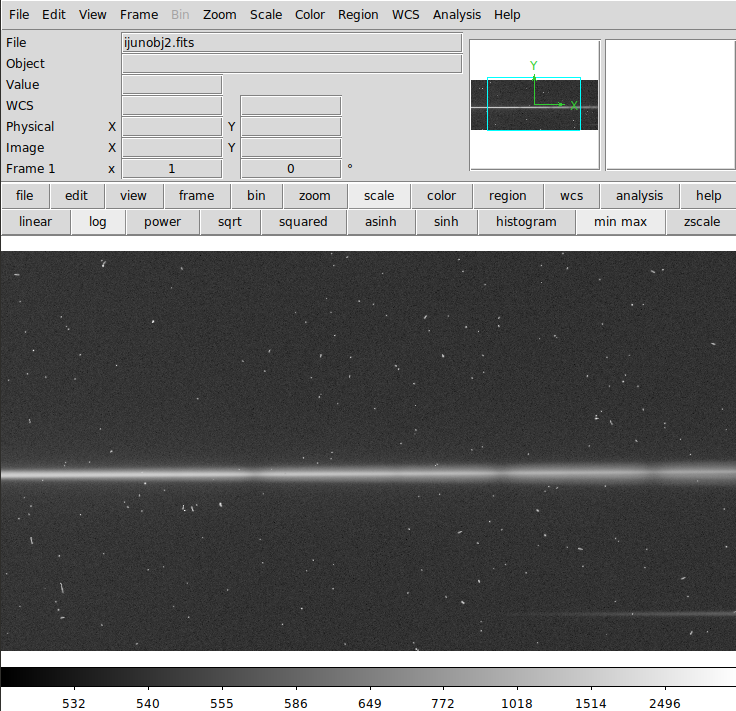
\includegraphics[scale=0.4]{iraf/dispersed object.png}
    \caption{Object}
    \label{fig:my_label}
\end{figure}

\begin{figure}[H]
    \centering
    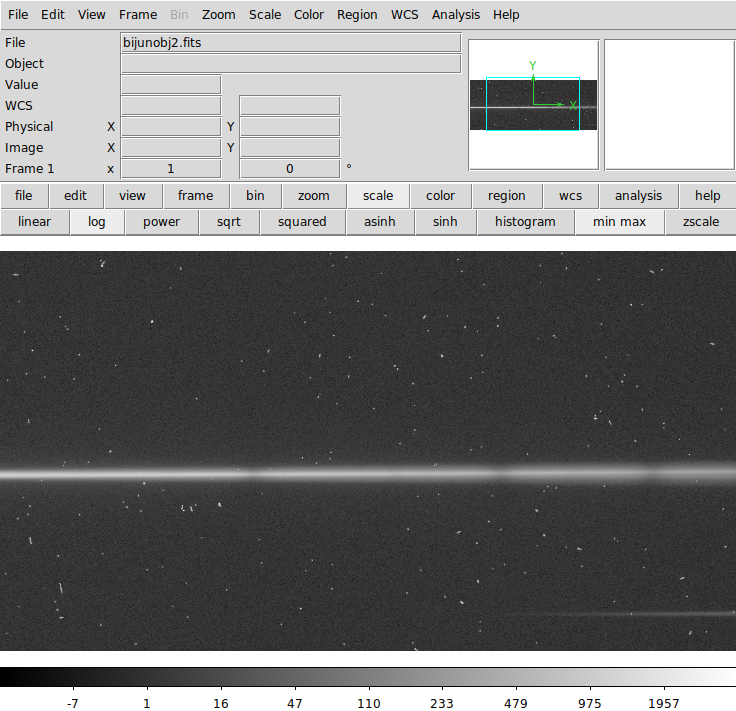
\includegraphics[scale=0.4]{iraf/dispersed b.png}
    \caption{Bias substracted Object}
    \label{fig:my_label}
\end{figure}

\begin{figure}[H]
    \centering
    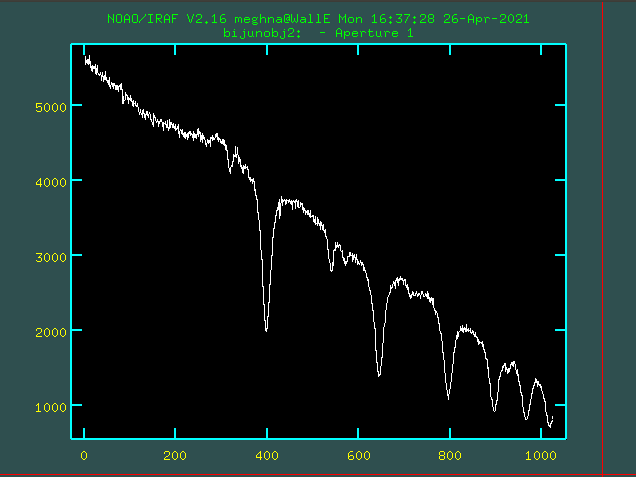
\includegraphics[scale=0.4]{iraf/ijunobj.png}
    \caption{Extracted spectra}
    \label{fig:my_label}
\end{figure}

\section{Conclusion}
The Object spectra is extracted using IRAF. Once the object spectra and lamp spectra are extracted, wavelength
calibration can be performed.

\section{References}
\begin{itemize}
    \item \href{http://ast.noao.edu/data/software}{http://ast.noao.edu/data/software}
    \item \href{https://iraf.net/}{https://iraf.net/}
    \item \href{https://iraf-community.github.io/}{https://iraf-community.github.io/}
\end{itemize}






\chapter{Wavelength calibration of the spectra using IRAF}
\section{Aim}
Calibrate the spectrum extracted using IRAF image reduction

\section{Theory}
The temperature, chemical composition, and intrinsic luminosity of a star are all contained in its spectrum. A
spectrograph is a device that collects and records astronomical spectra.The spectrograph divides or disperses
light from an object into its component wavelengths, allowing it to be recorded and analysed. An astronomer
can obtain a useful spectrum much faster with a $CCD$ than with a photographic plate, and he or she can even
obtain spectra from much fainter sources. For storage and examination, a $CCD$ spectra can be read directly to
a computer disc.
Having established the aperture and trace of the stellar spectrum, it behooves one to extract the comparison
spectrum in exactly the same manner and then identify the various lines and perform a smooth fit to the
wavelength as a function of pixel number along the trace. This is called wavelength calibration. The wavelength
calibration of the instrument is performed by scanning through the grating angles and measuring a spectrum
with known wavelengths. A comparison of the measured values of the wavelengths with the known values
constitutes a wavelength calibration of the spectrometer.

\section{Source and Tools}
\subsection{IRAF}
IRAF (Image Reduction and Analysis Facility) is a collection of software written at the National Optical Astronomy Observatory (NOAO) geared towards the reduction of astronomical images in pixel array form. This is primarily data taken from imaging array detectors such as CCDs.
    
\section{Procedure}
\begin{itemize}
    \item Open the extracted spectra in \emph{identify} tool using
        \begin{lstlisting}
        epar identify
        \end{lstlisting}
    edit the lines
         \begin{lstlisting}
        images = blamp.ms.fits
        .
        .
        coordli = linelist$fear.dat
        \end{lstlisting}
    \item In the opened window, click each spectrum line and enter its wavelength\\ Use the following commands to navigate the spectrum
        \begin{table}[h!]
            \centering
            \begin{tabular}{c|c}
                key & command \\\\
                \hline \\
                 \emph{Shift}+\emph{x} & zoom  \\
                 \emph{r} & exit zoom \\
                 \emph{m} & mark \\
                 \emph{d} & delete mark \\
                 \emph{u} & undo delete \\
                 
            \end{tabular}
            
            \label{tab:my_label}
        \end{table}
    \item Press \emph{f} to fit
    \item Enter \begin{lstlisting}
            :o 2
        \end{lstlisting} to specify order of fitting
    \item Press \emph{f} , \emph{q} , \emph{q} 
    \item Type \emph{yes} to save identified lines
    \item Refer lamp spectra to object spectra using \emph{refspec}
        \begin{lstlisting}
        epar refspec
        \end{lstlisting}
    \item Give proper input and reference files, then type
        \begin{lstlisting}
        :go
        \end{lstlisting} 
        Type \emph{yes} for all questions
    \item Use \emph{dispcor} to get the dispersion corelation from pixel to wavelength.
        \begin{lstlisting}
        epar dispcor
        \end{lstlisting}
    \item Give proper input and reference files, then type
        \begin{lstlisting}
        :go
        \end{lstlisting} 
        Type \emph{yes} for all questions
\end{itemize}

\section{Results}

\begin{figure}[H]
    \centering
    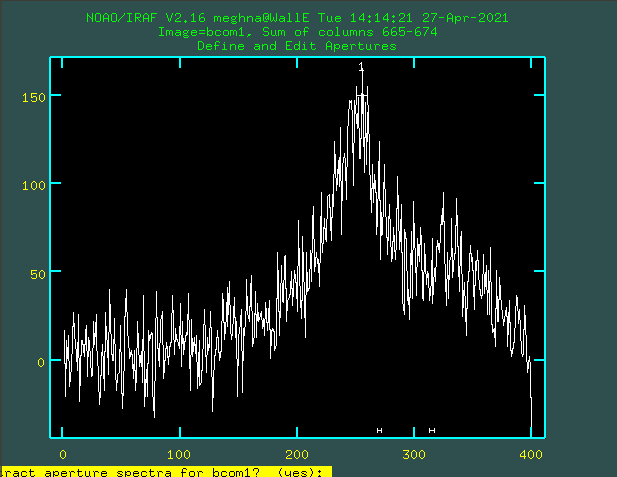
\includegraphics[scale=0.4]{iraf/lamp spectra.png}
    \caption{Lamp Spectra}
    \label{fig:my_label}
\end{figure}

\begin{figure}[H]
    \centering
    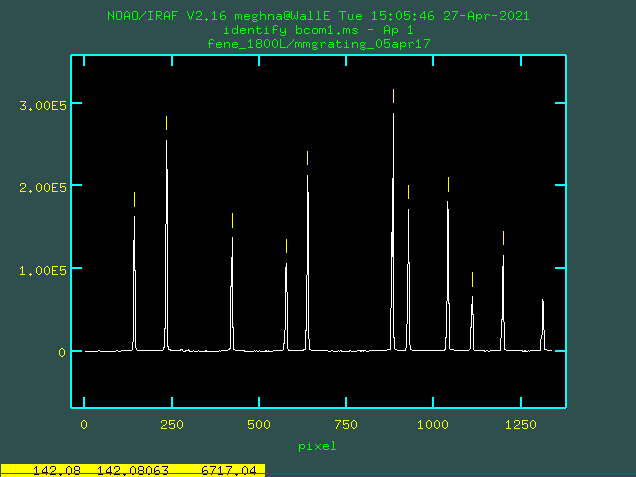
\includegraphics[scale=0.4]{iraf/marked lampspectra.png}
    \caption{Marked Lamp Spectra}
    \label{fig:my_label}
\end{figure}

\begin{figure}[H]
    \centering
    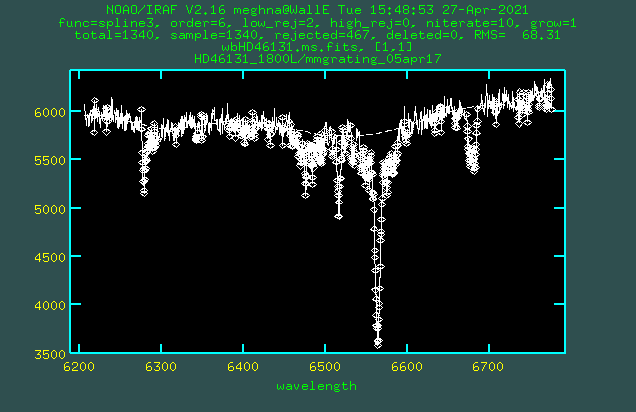
\includegraphics[scale=0.4]{iraf/wavelength calibrated.png}
    \caption{Wavelength Calibrated Spectra}
    \label{fig:my_label}
\end{figure}

\section{Conclusion}
The Object spectra and the lamp spectra are extracted using IRAF. Using the extracted object spectra and lamp
spectra, wavelength calibration is performed. Here pixel axis is converted to wavelength axis after wavelength
calibration using $Fe-Ar$ lamp spectra.

\section{References}
\begin{itemize}
    \item \href{http://ast.noao.edu/data/software}{http://ast.noao.edu/data/software}
    \item \href{https://iraf.net/}{https://iraf.net/}
    \item \href{https://iraf-community.github.io/}{https://iraf-community.github.io/}
\end{itemize}



\chapter{Normalization of Calibrated spectra and Finding Equivalent Width using IRAF}

\section{Aim}
To normalize the calibrated spectra and to find the equivalent width using IRAF image reduction software.

\section{Theory}
Normalization is usually achieved by fitting a low order function to the spectrum.By observing the standard
stars and summing the counts over the same band-passes used to calibrate the standards, one can associate
a count rate (as a function of wavelength) with the published fluxes. In practice, one uses a low order fit to
the observed counts per second and the spectro-photometric magnitudes for all of the standard stars, applying
a grey shift to reduce the effects of slit losses. Optionally one might try to derive a wavelength dependent
extinction curve with such data. Finally one corrects the observed data by the mean extinction curve and
applies the flux calibration to the data. The final spectrum is then in terms of either $f\lambda$ vs wavelength.

\section{Tools Used}
\begin{itemize}
    \item IRAF
    \newline
    IRAF (Image Reduction and Analysis Facility) is a suite of software developed at the National Optical Astronomy Observatory (NOAO) for pixel array reduction of astronomical images. Data from imaging array detectors, such as CCDs, is mainly used. It is compatible with all major mainframe and desktop operating systems.
    IRAF commands are organized into package structures. Additional packages may be added to IRAF. Packages may contain other packages. There are many packages available by NOAO and external developers often focusing on a particular branch of research or facility.Functionality available in IRAF includes the calibration of the fluxes and positions of astronomical objects within an image, compensation for sensitivity variations between detector pixels, combination of multiple images or measurement of the redshifts of absorption or emission lines in a spectrum.
\end{itemize}

\section{Procedure}
\begin{itemize}
    \item For normalizing the continuum of the object spectra use the     task \emph{continuum}
        \begin{lstlisting}
        epar continuum
        :go
        \end{lstlisting}
        Edit few parameters and provide input and output. Answer \emph{yes} in the IRAF terminal.
    \item In the new window that appears
        \begin{lstlisting}
        :o 6
        \end{lstlisting}
        press \emph{enter}
        press \emph{f} to fit and press \emph{q}
    \item To examine the continuum normalized wavelength calibrated       object spectra type
        \begin{lstlisting}
        splot cwbobject.ms.fits
        \end{lstlisting}
    \item In order to find the equivalent width and FWHM\\
          Press \emph{a} keeping on one end of the dip in the normalized spectra.\\
        Press \emph{a} again keeping on the other end of the dip in the normalized spectra.\\
        Press \emph{k}\\
        Press \emph{k} again.\\
        This gives the equivalent width and FWHM of the dip.
\end{itemize}

\section{Results}

\begin{figure}[H]
    \centering
    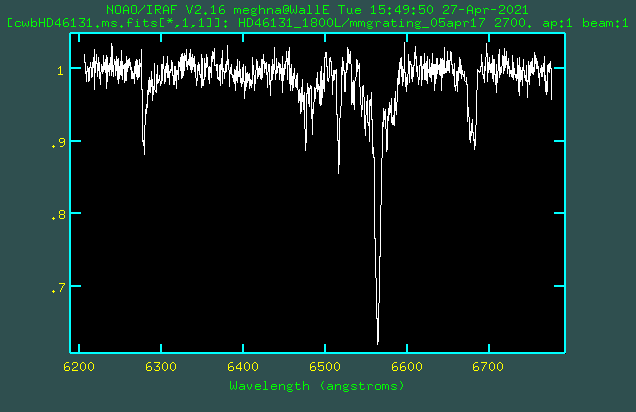
\includegraphics[scale=0.4]{iraf/normalized.png}
    \caption{Continuum Normalized Spectra}
    \label{fig:my_label}
\end{figure}

\begin{figure}[H]
    \centering
    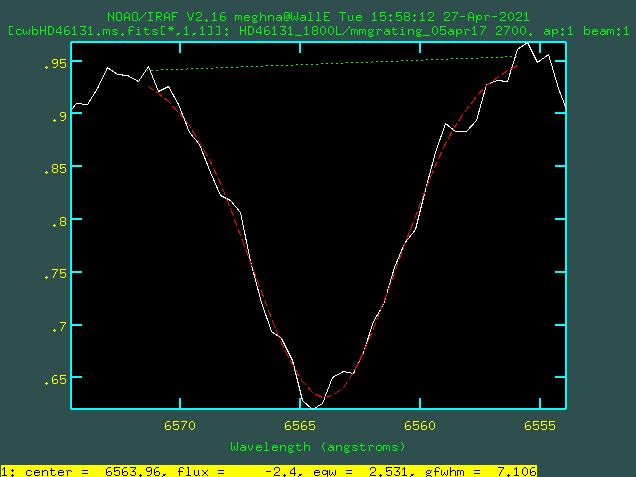
\includegraphics[scale=0.4]{iraf/equivalent width.png}
    \caption{Equivalent Width measured}
    \label{fig:my_label}
\end{figure}

\section{Conclusion}
The normalization of the wavelength calibrated object spectra is performed and the equivalent width is found
using IRAF image reduction software. The equivalent width and FWHM of the absorption dip in the spectra
is found to be 2.531 and 7.106 respectively and it shows $ H_\alpha $  absorption.

\section{References}
\begin{itemize}
    \item \href{http://ast.noao.edu/data/software}{http://ast.noao.edu/data/software}
    \item \href{https://iraf.net/}{https://iraf.net/}
    \item \href{https://iraf-community.github.io/}{https://iraf-community.github.io/}
\end{itemize}

\chapter{Hubble redshift distance relation using Project CLEA}

\section{Aim}
To find the relationship between the redshift in spectra of distant galaxies and the rate of the expansion of the universe using CLEA Program "Hubble Redshift Distance Relation".

\section{Theory}
The software for the CLEA Hubble Redshift Distance Relation laboratory exercise puts in control of a large optical telescope equipped with a TV camera and an electronic spectrometer. Using this equipment, one can determine the distance and velocity of several galaxies located in selected clusters around the sky. The redshift of a galaxy can be determined by comparing the measured wavelength of a specific line or set of lines to the known wavelength of the line(s) when the emitter or absorber is at rest. Here we use the K and H lines of Ca II with rest wavelengths of $3933.7A^0$ and $3968.5A^0$ respectively. The recessional velocity v of the galaxy is then given by
\begin{equation}
    v=\frac{c*(\lambda_{obs}-\lambda_{rest})}{\lambda_{rest}}
\end{equation}
where $lambda_{rest}$ is the rest wavelength of the line given above, $\lambda_{obs}$ is the measured wavelength of the line from the galaxy’s spectrum, and $c=2.99792 × 10^5 km/s$.
\newline
To find the Hubble constant, we also need to determine the distance to the galaxies. To do this we assume that all of the galaxies in this sample have an absolute magnitude of $M=-22$. From the apparent magnitude(m) of the galaxy we can determine it's distance using the distance modulus equation,
\begin{equation}
    d=10^{0.2*(m-M+5)}
\end{equation}
From recessional velocities of the galaxies and their distances, one can find the Hubble constant from the Hubble’s law equation
\begin{equation}
    v= H_0*d
\end{equation}
Once we have the Hubble constant calibrated by fitting a line to the measured velocities and distances for a sample of galaxies, we can use the relation directly to find the distance to other galaxies.  Assuming the Hubble constant has been constant throughout the lifetime of the universe we can also determine the age of the universe using the equation
\begin{equation}
    t=d/v=1/H_0
\end{equation}
\newline

\section{Tools used}
\begin{itemize}
    \item PROJECT CLEA
    \newline
    Project CLEA a contemporary laboratory experience in astronomy develops laboratory exercises that illustrate modern astronomical techniques using digital data and color images. Each CLEA laboratory exercise includes a dedicated computer program. The technical guides describe file formats, user-settable options, and algorithms used in the programs.
\end{itemize}

\section{Procedure}
\begin{itemize}
    \item  Open the Hubble Redshift program by double clicking on the CLEA hub icon in the Astro121 folder. Select Log In from the menu bar, and enter name and the lab table number. Click OK when ready. The title screen appears.
    \item Select File…Run from the menu bar to begin the exercise. The screen shows the control panel and view
    window as found in the “warm room” at the observatory. Open the dome by clicking on the Dome button. Locate the Monitor button on the control panel and note its status, i.e. finder scope.
    \item Turn on the tracking by clicking the Tracking button. The telescope will now track in sync with the stars.
    \item Select a field of view. To review the fields of study for tonight’s observing session, select Field… from the menu bar at the top of the control panel. The items you see listed are the fields that contain the objects we have selected to study tonight.
    \item Select an object to study (one from each field of view).
    \item Find a galaxy and slew the telescope using the N, S, E, W buttons so that the galaxy is inside the red finder window.
    \item Click on the Monitor button to change the view from the Finder Scope to the Spectrometer. . Use the directional buttons (N, S, E or W), to slew the telescope to carefully
    position, in the slit, the object you intend to use to collect data. After positioning the galaxy accurately in the slit, click on the Take Reading button. Press Start/Resume Count. When the Signal/Noise reaches 15 or more, click the Stop Count button. The computer will plot the spectrum with the available data. Find the H and K lines of calcium.
    \item Record the object name, apparent magnitude, signal/noise, and the measured wavelength of the H and K lines of calcium. Then choose a second galaxy in the same galaxy field and repeat these steps. Go to Change Field on the menu and record data for two galaxies in each of the 5 galaxy fields.
    \item Calculate the distance d and velocity v for the above saved data using the equations above.
    \item Plot a Hubble diagram by graphing the velocity of a galaxy in km/sec (y-axis) vs. the distance in mega parsecs (x-axis). The slope of this straight line graph gives the Hubble constant and from that the age of the universe.
\end{itemize}

\section{Results}

\subsection{Observations}
\begin{center}
    \begin{tabular}{c|c|c|c}
        Object name & Apparent magnitude & K-line & H-line  \\ \hline 
        36773&	15.8&	4125.5&	4162 \\
        36747&	15.6&	4130.83	&4167.33 \\
        36805&	15.4&	4133.33&	4169.83 \\
        ngc 4874&	12.9&	4027.67&	4064.17 \\
        ngc 4889&	12.5&	4020&	4056.5 \\
        51976&	17.9&	4445.83&	4482.33 \\
        51975&	18.5&	4455&	4491.5 \\
        54876&	16&	4206&	4242.5 \\ 
    \end{tabular}
\end{center}

\subsection{Calculations}
\subsubsection{Distance calculation}
\begin{center}
    \begin{tabular}{c|c|c|c}
        Object name & Apparent magnitude & Distance (pc) & Distance(Mpc)  \\ \hline 
        36773 &	15.8 &	363078054.8 & 363.0780548 \\
        36747 &	15.6 &	331131121.5 & 331.1311215 \\
        36805 &	15.4 &	301995172 & 301.995172 \\
        ngc 4874 &	12.9 &	95499258.6 & 95.4992586 \\
        ngc 4889 &	12.5 &	79432823.47 & 79.43282347 \\
        51976 &	17.9 &	954992586 & 954.992586 \\
        51975 &	18.5 &	1258925412 & 1258.925412 \\
        54876 &	16 & 398107170.6 & 398.1071706 \\
    \end{tabular}
\end{center}

\subsubsection{Velocity calculation}
\begin{center}
    \begin{tabular}{c|c|c|c|c|c|c|c}
        Obj & K-line& H-line &\Delta K-line&\Delta H-line& v_k (km s^{-1})& v_h (km s^{-1}) & v_{avg} (km s^{-1})\\ \hline
        36773&	4125.5&	4162 & 191.83 & 193.5 & 14629.84948 & 14627.69308 & 14628.77128 \\
        36747&	4130.83&	4167.33 & 197.16 & 198.83 & 15036.34011 & 15030.6161 & 15033.47811 \\
        36805&	4133.33&	4169.83 & 199.66 & 201.33 & 15227.00176 & 15219.60438 & 15223.30307 \\
        ngc 4874&	4027.67&	4064.17 & 94 & 95.67 & 7168.877918 & 7232.203603 & 7200.540761 \\
        ngc 4889&	4020&	4056.5 & 86.33 & 88 & 6583.927986 & 6652.387552 & 6618.157769 \\
        51976&	4445.83&	4482.33 & 512.16 & 513.83 & 39059.7076 & 38843.13973 & 38951.42366 \\
        51975&	4455&	4491.5 & 521.33 & 523 & 39759.05452 & 39536.34875 & 39647.70163 \\
        54876&	4206&	4242.5 & 272.33 & 274 & 20769.1545 & 20713.11579 & 20741.13515 \\
    \end{tabular}
\end{center}

\newpage

\subsubsection{Hubbles constant calculation}
\begin{center}
    \begin{tabular}{c|c|c|c}
        Object name & Distance (Mpc) & Velocity (km s^{-1}) & H_0 (km s^{-1} Mpc^{-1}) \\ \hline
        36773 & 363.0780548 & 14628.77128 & 40.29098176 \\
        36747 & 331.1311215 & 15033.47811 & 45.40037807 \\
        36805 & 301.995172 & 15223.30307 & 50.40909418 \\
        ngc 4874 & 95.4992586 & 7200.540761 & 75.39891792 \\
        ngc 4889 & 79.43282347 & 6618.157769 & 83.31766995 \\
        51976 & 954.992586 & 38951.42366 & 40.78714771 \\
        51975 & 1258.925412 & 39647.70163 & 31.49328885 \\
        54876 & 398.1071706 & 20741.13515 & 52.09937595 \\
    \end{tabular}
\end{center}

\begin{center}
    \begin{figure}[H]
        \centering
        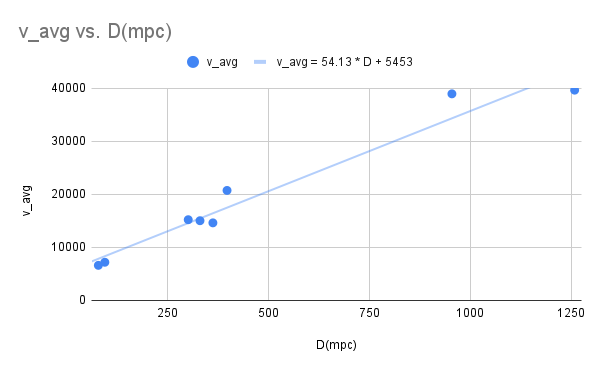
\includegraphics[scale = 0.7]{v_avg vs. D(mpc).png}
        \caption{Hubble's constant plot}
        \label{fig:my_label}
    \end{figure}
\end{center}

\begin{center}
    Average $H_0$ is $52.3996068$ $km s^{-1} Mpc^{-1}$ \\
    Velocity of galaxy at 800 Mpc is $41919.68544$ $km s^{-1}$ \\
    Age of Universe is $5.8887417x10^{17}$ $s$ or $18$ $GYr$
\end{center}

\section{Conclusion}
Using CLEA , velocity and distance of various galaxies were calculated , then plotted . The Hubble's Constant value is calculated as $52.3996068$ $km s^{-1} Mpc^{-1}$ and the Age of the Universe is calculated as $18$ $GYr$

\section{References}
\begin{itemize}
    \item \href{http://public.gettysburg.edu/~marschal/clea/CLEAhome.html}{http://public.gettysburg.edu/~marschal/clea/CLEAhome.html}
    \item \href{http://public.gettysburg.edu/~marschal/clea/clea-products/manuals/Hubbl-ug.pdf}{http://public.gettysburg.edu/~marschal/clea/clea-products/manuals/Hubbl-ug.pdf}
    \item \href{http://www.ifa.hawaii.edu/~meech/education/clea.html}{http://www.ifa.hawaii.edu/~meech/education/clea.html}
\end{itemize}



\chapter{Read and plot an image from a FITS file}

\section{Aim}
Read a FITS file. Open the image stored in the FITS file and plot it and display it.

\section{Theory}
Flexible Image Transport System (FITS) is an open standard defining a digital file format useful for storage, transmission and processing of data: formatted as multi-dimensional arrays (for example a 2D image), or tables. FITS is the most commonly used digital file format in astronomy. The FITS standard was designed specifically for astronomical data, and includes provisions such as describing photometric and spatial calibration information, together with image origin metadata.
Image metadata is stored in a human-readable ASCII header. The information in this header is designed to calculate the byte offset of some information in the subsequent data unit to support direct access to the data cells. Each FITS file consists of one or more headers containing ASCII card images that carry keyword/value pairs, interleaved between data blocks. The keyword/value pairs provide information such as size, origin, coordinates, binary data format, free-form comments, history of the data, and anything else the creator desires: while many keywords are reserved for FITS use, the standard allows arbitrary use of the rest of the name-space.
FITS is also often used to store non-image data, such as spectra, photon lists, data cubes, or structured data such as multi-table databases. A FITS file may contain several extensions, and each of these may contain a data object. For example, it is possible to store x-ray and infrared exposures in the same file.


\section{Tools used }
\begin{itemize}
    \item Python 
    \item \emph{astropy} package: \\
        The \emph{astropy} package contains key functionality and common tools needed for performing astronomy and astrophysics with Python. It is at the core of the Astropy Project, which aims to enable the community to develop a robust ecosystem of affiliated packages covering a broad range of needs for astronomical research, data processing, and data analysis.
        
        \begin{itemize}
            \item \emph{astropy.utils} \\
                The \emph{astropy.utils} package contains general-purpose utility functions and classes. Examples include data structures, tools for downloading and caching from URLs, and version intercompatibility functions.
                This functionality is not astronomy-specific, but is intended primarily for use by Astropy developers. It is all safe for users to use, but the functions and classes are typically more complicated or specific to a particular need of Astropy.
                Because of the mostly standalone and grab-bag nature of these utilities, they are generally best understood through their docstrings, and hence this documentation generally does not have detailed sections like the other packages. The exceptions are 
                IERS data access (\emph{astropy.utils.iers})
                Downloadable Data Management (\emph{astropy.utils.data})
            
            \item \emph{astropy.io.fits} \\
                The \emph{astropy.io}.fits package provides access to FITS files. FITS (Flexible Image Transport System) is a portable file standard widely used in the astronomy community to store images and tables.
        \end{itemize}
    \item \emph{matplotlib} package \\
        Matplotlib is a comprehensive library for creating static, animated, and interactive visualizations in Python.
        \begin{itemize}
            \item \emph{matplotlib.pyplot} is a state-based interface to matplotlib. It provides a MATLAB-like way of plotting.
            pyplot is mainly intended for interactive plots and simple cases of programmatic plot generation:
        \end{itemize}
        
\end{itemize}

\section{Procedure}
\subsection{Setting Up}
\subsubsection{Input}
\begin{enumerate}
    \item Set up \emph{matplotlib} and use a nicer set of plot parameters
        \begin{lstlisting}
        import matplotlib.pyplot as plt
        from astropy.visualization import astropy_mpl_style
        plt.style.use(astropy_mpl_style)
        \end{lstlisting}
    \item Download the example FITS files used by this example:
        \begin{lstlisting}
        from astropy.utils.data import get_pkg_data_filename
        from astropy.io import fits
        image_file = get_pkg_data_filename('tutorials/FITS-images/
            HorseHead.fits')
        \end{lstlisting}
    \item Use \emph{astropy.io.fits.info()} to display the structure of the file:
        \begin{lstlisting}
        fits.info(image_file)
        \end{lstlisting}
\end{enumerate}
    
\subsubsection{ Output}
\begin{lstlisting}
Filename: /home/docs/.astropy/cache/download/url/
    ff6e0b93871033c68022ca026a956d87/contents
No.    Name      Ver    Type      Cards   Dimensions   Format
0  PRIMARY       1 PrimaryHDU     161   (891, 893)   int16 
1  er.mask       1 TableHDU        25   1600R x 4C   [F6.2, F6.2, F6.2, F6.2]
\end{lstlisting}

\subsection{Extracting Image Data}
\subsubsection{Input}

\begin{enumerate}
    \item Generally the image information is located in the Primary HDU, also known as extension 0. Here, we
    use \emph{astropy.io.fits.getdata()} to read the image data from this first extension using the keyword
    argument \emph{ext=0}
        \begin{lstlisting}
        image_data = fits.getdata(image_file, ext=0)
        \end{lstlisting}
    \item The data is now stored as a 2D numpy array. Print the dimensions using the shape attribute
        \begin{lstlisting}
        print(image_data.shape)
        \end{lstlisting}
\end{enumerate}

\subsubsection{Output}
\begin{lstlisting}
    (893, 891)
\end{lstlisting}

\subsection{Plotting Image}
\subsection{Input}
Display the image data:
    \begin{lstlisting}
        plt.figure()
        plt.imshow(image_data, cmap='gray')
        plt.colorbar()
        plt.show()
    \end{lstlisting}
    
    
\subsubsection{Output}
\begin{figure}[H]
    \centering
    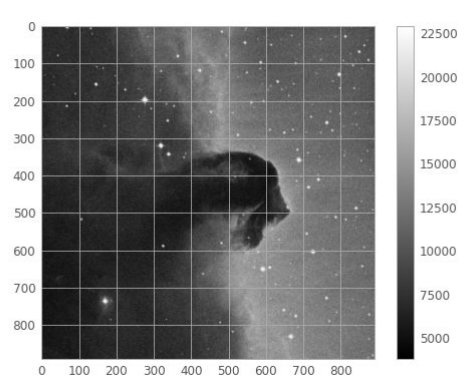
\includegraphics[scale = 0.5]{horsey.png}
    \caption{}
    \label{fig:my_label}
\end{figure}

\section{Conclusion}
 We were able to successfully read a FITS file , plot the image stored in the FITS file and display it.
 
\section{References}
\begin{itemize}
    \item FITS File Handling (astropy.io.fits) — Astropy v4.2.1 \\ \href{https://docs.astropy.org/en/stable/io/fits/index.html#module-astropy.io.fits}{https://docs.astropy.org/en/stable/io/fits/index.html#module-astropy.io.fits}
    \item Astropy Core Package Utilities (astropy.utils) — Astropy v4.2.1 \\
    \href{https://docs.astropy.org/en/stable/utils/index.html#module-astropy.utils.data}{https://docs.astropy.org/en/stable/utils/index.html#module-astropy.utils.data}
    \item MatPlotLib/Pyplot \\ \href{https://matplotlib.org/api/_as_gen/matplotlib.pyplot.html#module-matplotlib.pyplot}{https://matplotlib.org/api/_as_gen/matplotlib.pyplot.html#module-matplotlib.pyplot}
\end{itemize}
\end{document}
